%
% File emnlp2018.tex
%
%% Based on the style files for EMNLP 2018, which were
%% Based on the style files for ACL 2018, which were
%% Based on the style files for ACL-2015, with some improvements
%%  taken from the NAACL-2016 style
%% Based on the style files for ACL-2014, which were, in turn,
%% based on ACL-2013, ACL-2012, ACL-2011, ACL-2010, ACL-IJCNLP-2009,
%% EACL-2009, IJCNLP-2008...
%% Based on the style files for EACL 2006 by 
%%e.agirre@ehu.es or Sergi.Balari@uab.es
%% and that of ACL 08 by Joakim Nivre and Noah Smith

\documentclass[11pt,a4paper]{article}
\usepackage[hyperref]{emnlp2018}
\usepackage{times}
\usepackage{latexsym}

\usepackage{url}

%\aclfinalcopy % Uncomment this line for the final submission
%\def\aclpaperid{***} %  Enter the acl Paper ID here

%\setlength\titlebox{5cm}
% You can expand the titlebox if you need extra space
% to show all the authors. Please do not make the titlebox
% smaller than 5cm (the original size); we will check this
% in the camera-ready version and ask you to change it back.

\newcommand\BibTeX{B{\sc ib}\TeX}
\newcommand\confname{EMNLP 2018}
\newcommand\conforg{SIGDAT}

\title{Instructions for \confname{} Proceedings}

\author{First Author \\
  Affiliation / Address line 1 \\
  Affiliation / Address line 2 \\
  Affiliation / Address line 3 \\
  {\tt email@domain} \\\And
  Second Author \\
  Affiliation / Address line 1 \\
  Affiliation / Address line 2 \\
  Affiliation / Address line 3 \\
  {\tt email@domain} \\}

\date{}

\begin{document}
\maketitle

\begin{abstract}
	TBD
\end{abstract}
\section{Introduction}

Relation extraction (\RE) aims at identifying relations between pairs of entities from raw text, and its success can benefit  many knowledge base (\KB) related tasks like \KB population, question answering (\QA) and etc~\cite{suchanek2013advances}.

In the literature, \RE is usually investigated in the distant supervision (\DS) paradigm, where datasets are automatically constructed by aligning existing \KB \emph{(subject, relation, object)} triples with a large corpus, and considers sentences containing the subject and object entity in a triple as evidence for the corresponding relation~\cite{riedel2010modeling}.
To alleviate the sentence level noise in the automatically constructed dataset, \RE is often considered in the multi-instance learning (\MIL) framework where all the sentences containing the target subject and object are packed into a \textbf{\emph{sentence bag}}, and relation extractors take in these sentences to predict the relations for the entity pair. 
Following this framework, Zeng et al.~\shortcite{zeng2015distant} uses piecewise convolutional neural network (\PCNN) to handle the extraction task, Lin et al.~\shortcite{lin2016neural} introduces attention mechanism for better noise tolerance,
%methods like graphic model~\cite{surdeanu2012multi}, neural network~\cite{lin2016neural} have been successfully used,
Ye et al.~\shortcite{ye2017jointly} makes further improvements by learning co-occurrence tendency between relations via learning to rank.
%In the literature, \RE is usually investigated in a classification style, where the classifier takes in sentences containing the mentions of the target entity pair, and output the predicted relations between them~\cite{hoffmann2011knowledge,surdeanu2012multi,zeng2015distant,lin2016neural}.

Typically, most existing relation extractors relies only on input sentences to make predictions, and ignores the constraints required by each relation.
Take the relation \emph{Capital} for example, it expects its subject to be a \underline{country} and its object to be a \underline{city}.
And in most cases, it also expects a city to be the capital of only one country.
This kind of constraints can help us identify inconsistent predictions and thereby improve the extraction results.

However, properly utilizing these clues is non-trivial, since many \KBs do not have a well-defined typing system or a cardinality specification for relations.
Chen et al~\shortcite{chen2014encoding} evades this difficulty by implicitly mining such requirements from data.
Specifically, while collecting cardinality requirements directly from data, they evades the tricky argument type constraints by collecting relations pairs that have the same subject or object type instead, which do not require a concrete specification for argument type.
Then, they use  integer linear programming (\ILP) to resolve the predictions that are inconsistent regarding the constraints.
However, since \ILP operates at the post-processing phase, their method typically requires more time during prediction.
Besides, since \ILP does not change the prediction scores of the base model, it tends to leave the predictions corrected by the constraints with low scores, which hurts the performance in terms of the precision-recall curve criterion.
%and introduces high delay to the use of the extraction results since we need to wait for all the extractions to complete before the ILP step.
%which is inappropirate for downstream applications like \QA that need to use the \RE result immediately when 
%clw's model operates on sentence level, which kind of deviates the multi-instance learning procedure, and therefore may introduce some performance drop.

To overcome the problems of \ILP, we propose to incorporate these constraints by introducing an additional loss term to penalize inconsistent predictions during training.
%which improves the prediction ability of the base model, and the prediction phase incurs no extra costs.
Specifically, we consider the type and cardinality constraints as propositional logic constraints, and use the semantic loss framework~\cite{xu2017semantic} to convert them into a loss term.
Compared to other methods of enforcing logical constraints like the teacher-student network~\cite{hu2016harnessing} that relies on fuzzy relaxation of the constraints, semantic loss possesses the precise meaning of the constraints and is fully differentiable since it directly use the predicted probability to construct the loss.
In this way, the base model is encouraged to find more textual clues when detecting conflicts, which leads to better prediction ability of the model, and the prediction phase incurs no extra costs.
%the classification boundary is made more discriminative and therefore lead to better generalization ability of the model.
Further, since we only add a loss term to the base model, our method is plug-and-play for most relation extraction models.
% Further, the extra cost only reside in the training procedure, and the test is as efficient as before.

We conduct experiments on both English and Chinese datasets,
and the experimental results show that our method can clearly improve the base model, and delivers superior performance compared to the \ILP method.
%Mention the simplified version?


\section{Our Approach}
%Briefly introduce the whole framework, and refer to each subsection one by one.
In this section, we describe a novel loss term that incorporates the type constraints and the cardinality constraints required by each relation,
which significantly increases the quality of relation extraction results with only moderate extra cost during training.
First, we briefly introduce our base relation extraction model (Sec.~\ref{sec:base_model}).
Then we describe our constraints in detail (Sec.~\ref{sec:constraints}) and how to incorporate these constraints during training (Sec.~\ref{sec:loss_term}).
%Before delving into the details of our method (Sec.~\ref{sec:loss_term}), we first briefly introduce our base relation extraction model (Sec.~\ref{sec:base_model}), and the constraints that we will use (Sec.~\ref{sec:constraints}).





\subsection{Base Model}
\label{sec:base_model}
%Briefly introduce the base model (PCNN).
Although our loss term is compatible to most existing relation extractors, in this paper, we take the attentive piecewise convolutional neural network (\APCNN)~\cite{lin2016neural} as our base model, which is currently one of the most widely used extractor in the relation extraction task.

Specifically, \APCNN operates in the \MIL framework that takes in all the sentences mentioning the target subject and object, and output the relations between these two entities.
We first use the piecewise convolutional neural network (\PCNN)~\cite{zeng2015distant} to obtain the embedding of each sentence.
Then, an attention layer is applied to these sentence embeddings to selectively aggregate them into a sentence bag embedding, which is then fed to a softmax classifier to generate the predicted relation distribution, $\bm{p}$.

%First, we concatenate the word embeddings and position embeddings of each word in one sentence, the position embeddings indicates how close each word is to head or tail entities. Then, we use a convolutional layer with window size 3, a max pooling layer and a non-linear layer to merge all these features and get the representation of one sentence.Then a selective attention is done over a bag of sentences to get the bag representation.


\subsection{Relation Constraints}
\label{sec:constraints}
%Describe clw's argument type constraints
%只介绍两类规则,一类是不同关系主体客体的约束,一类是相同关系主体客体的约束

%\cite{xu2017semantic}  encodes the symbolic knowledge in Boolean logic, and derives a semantic loss to make the neural network automatically learn the symbolic knowledge. Their experiments show that the semantic loss helps to reduce the constraint violation and gives significant practical improvements in semi-supervised classification. 

%Inspired by their work, we encode the constraints in \cite{chen2014encoding} to boolean logic, and add a semantic loss to the neural network.

Following Chen et al.~\shortcite{chen2014encoding}, our relation constraints are defined over each combination of two entity pairs: ($subj_1$, $obj_1$), ($subj_2$, $obj_2$).
We derive type constraints and cardinality constraints from an existing KB to implicitly capture the expected type and cardinality requirements for the arguments of a relation. 
%\paragraph{Implicit Argument Types Inconsistencies:}
\paragraph{Type Constraint}
%Due to the lack of well-defined typing systems in most \KBs, determining the expected argument type of each relation with appropriate granularity is usually a hard problem.
%Generally, the argument types of the correct predictions should be consistent with each other.
Similar to Chen et al.~\shortcite{chen2014encoding}, we also use entity sharing between relations to implicitly capture the expected argument type of each relation.
Specifically, if the subject set of relation $R_1$ in \KB has a large intersection with those in $R_2$, then we consider $R_1$ and $R_2$ have the same expected subject type. 
We thereby collect relation paris that have the same subject type ($\bm{C}^{ts}$), object type ($\bm{C}^{to}$), and relation pairs whose subject type of $R_1$ is the same as the object type of $R_2$ ($\bm{C}^{tso}$).
%finding relation pairs that can share the same subject ($C^s$), object ($C^o$), and those where the subject of one relation can be the object of the other ($C^{so}$).
Then, $\bm{C}^{ts}$, $\bm{C}^{to}$ and $\bm{C}^{tso}$ represents the constraints that we expect ($r_1$, $r_2$) of the predicted ($subj_1$, $r_1$, $obj_1$),  ($subj_2$, $r_2$, $obj_2$) pairs fall into $\bm{C}^{ts}$ when $subj_1=subj_2$, $\bm{C}^{to}$ when $obj_1=obj_2$ and $\bm{C}^{tso}$ when when $subj_1=obj_2$ respectively.
%Then, we expect the relations of all pairs of predicted \emph{(subject, relation, object)} triples to fall into $\bm{C}^{ts}$, $\bm{C}^{to}$ or $\bm{C}^{tso}$ when they share the same entity in either subject or object.
The idea is that, if the predicted relations of two triples require the same entity to belong to different types, then at least one of the prediction must be wrong.
%The idea is that, take $C^s$ for example, if the subject set of relation $R_1$ has a large intersection with those in $R_2$ (($R_1$, $R_2$) lies in $C^s$ ), then the expected subject type of $R_1$ and $R_2$ are likely to be the same. Therefore, if a pair of predicted relation $R_1'$ and $R_2'$ for two entity pairs share the same subject, which implies $R_1'$ and $R_2'$ have the same expected subject type, then ($R_1'$, $R_2'$) must lie in $C^s$. 
%\red{luo: Hard to explain this clearly given limited space. Maybe we can delete the intuition part.}

% if the predicted relations of two entity pairs require the same entity to belong to mutually-exclusive types, then at least one of the prediction must be wrong.
%Take \textless USA, New York\textgreater and \textless USA, Washington D.C.\textgreater as an example. We couldn't predict two relations for them which has different Subject types, such as $ LargestCity $ and $ LocationCity $.

%\paragraph{Violations of Arguments' Uniqueness:}
\paragraph{Cardinality Constraint}
Given a subject (or object), some relations should only have one object (or subject).
For example, the relation \emph{Capital} would expect only one object for a given subject.
Following this observation, we collect relations that can have multiple objects ($\bm{C}^{co}$) or subjects ($\bm{C}^{cs}$),
and $\bm{C}^{co}$ (or $\bm{C}^{cs}$) represents the constraint that we expect the relation of the predicted ($subj_1$, $r$, $obj_1$),  ($subj_2$, $r$, $obj_2$) pairs fall into $\bm{C}^{co}$ (or $\bm{C}^{cs}$) when $subj_1=subj_2 \land obj_1\neq obj_2$ (or $subj_1\neq subj_2 \land obj_1=obj_2$)
%expect the predicted relations that have multiple objects (or subjects) for a given subject (or object) to fall into $\bm{C}^{co}$ (or $\bm{C}^{cs}$).

% For example, given USA as the subject of the relation Capital, we can only accept one possible object, because there is great chance that a country only have one capital.

\iffalse
\begin{table}[!t]  
	\centering  
	\scriptsize  
	\begin{tabular}{ll}  
		\\[-2mm]  
		\hline  
		\hline\\[-2mm]
		\vspace{1mm}
		%\multicolumn{2}{|c|}{?}\\
		Details about Argument Type Constraints in \cite{chen2014encoding}\\
		\hline\\[-2mm]  
		\vspace{1mm}
		Given two entity tuples $(s_1, r_1, o_1), (s_2, r_2, o_2)$:\\ 
		\vspace{1mm} 
		Subj-Cons      &   \tabincell{l}{$s_1 \neq s_2 \quad when \quad r_1 \neq r_2$}\\  
		\vspace{1mm}  
		Obj-Cons       &   \tabincell{l}{$o_1 \neq o_2 \quad when \quad r_1 \neq r_2$}\\  
		\vspace{1mm}  
		Subj-Obj-Cons  &   \tabincell{l}{$s_1 \neq o_2 \vee o_1 \neq s_2 \quad when \quad r_1 \neq r_2$}\\  
		\vspace{1mm}  
		Subj-Uni       &   \tabincell{l}{$s_1 \neq s_2 \quad when \quad r_1 = r_2 \wedge o_1 = o_2$}\\  
		\vspace{1mm}  
		Obj-Uni        &   \tabincell{l}{$o_1 \neq o_2 \quad when \quad r_1 = r_2 \wedge s_1 = s_2$}\\  
		\hline  
		\hline  
	\end{tabular} 
	\caption{Argument Type Constraints}  
	\label{tab:notations}  
\end{table} 
\fi
\iffalse
Given two entity tuples $(s_1, r_1, o_1), (s_2, r_2, o_2)$: 

Subj-Cons:$s_1 \neq s_2 \quad when \quad r_1 \neq r_2$
	
Obj-Cons:$o_1 \neq o_2 \quad when \quad r_1 \neq r_2$
	
Subj-Obj-Cons:$s_1 \neq o_2 \vee o_1 \neq s_2 \quad when \quad r_1 \neq r_2$

Subj-Uni:$s_1 \neq s_2 \quad when \quad r_1 = r_2 \wedge o_1 = o_2$

Obj-Uni:$o_1 \neq o_2 \quad when \quad r_1 = r_2 \wedge s_1 = s_2$
\fi
%Subj-Cons: $r_1$ and $r_2$ can't have same subject. Obj-Cons means $r_1$ and $r_2$ can't have same object. Subj-Obj-Cons means $r_1$'s subject can't be $r_2$'s object or $r_2$'s subject can't be $r_1$'s object. Subj-Uni means if $r_1$ equals $r_2$, 


\subsection{Incorporating  Constraints for Training}
\label{sec:loss_term}
In this section, we demonstrate our method of converting the relation constraints into a loss term using the semantic loss framework~\cite{xu2017semantic}.
We also make suitable modifications to speed up the training process with only minor drop in prediction ability.

\paragraph{Relation Constraint Loss}
%Describe semantic loss, and how to encode clw's constraints into semantic loss.
Semantic loss is a general framework that can encode a propositional logic constraints as a loss term in a principled way.
%and derive a semantic loss to make the neural network automatically learning the symbolic knowledge. 
%This loss function captures how close the neural network is to satisfying the constraints on its output. 
Concretely, the semantic loss $L^{s}(\bm{C}, \bm{p})$ is defined as:
%For example, the semantic loss between an exactly-one constraint $\alpha$ and a neural net output vector $p$ captures how close the prediction $p$ is to having exactly one output set to true(1), and all false(0), regardless of which output is correct.
%We desire our semantic loss $L^{s}(\alpha, p)$ to be proportional to the negative log-probability of $\alpha$ being satisfied when sampling values according to $p$. More formally,
%In \cite{xu2017semantic}, the semantic loss function is formed as follows,
\begin{equation}
\label{seq:semantic_loss}
	L^{s}(\bm{C}, \bm{p}) = -log\sum\limits_{\bm x\models\bm{C}}\prod\limits_{i:\bm x\models X_i}p_i\prod\limits_{i:\bm x\models \neg X_i}(1-p_i)
\end{equation}
%over variables $\bm X=\{X_1,...,X_n\}$, and a vector of probabilities $p$, where $p_i$ denotes the predicted probability of variable $X_i$: 
where $\bm{C}$ is the set of propositional logic constraints defined over variables $\bm{X}$,
$p_i$ is the predicted probability of $X_i$,
$\bm x \models \bm{C}$ refers to the assignment $\bm x$ of variables $\bm X$ that satisfies constraints in $\bm{C}$,
and $i:\bm x \models X_i$ (or $i:\bm x\models \neg X_i$) refers to all the indices $i$ where $X_i$ is set to true (or false) in assignment $\bm x$.

As for our type constraints, the variables $\bm{X}\in \{0,1\}^{2R}$, where $R$ is the number of relations, are defined over a pair of  relations ($r_1$, $r_2$) which are assigned to 2 entity pairs ($subj_1$, $obj_1$) and ($subj_2$, $obj_2$) respectively.
Specifically, $X_i\in \bm{X}_{1...R}$ equals 1 only when $r_1$ is the $i^{th}$ relation,
and $X_{R+i}\in \bm{X}_{R+1...2R}$ equals 1 only when $r_2$ is the $i^{th}$ relation.
We thereby define three semantic loss terms: $m^{ts}L^{s}(\bm{C}^{ts}, \bm{p})$, $m^{to}L^{s}(\bm{C}^{to}, \bm{p})$, $m^{tso}L^{s}(\bm{C}^{tso}, \bm{p})$, where $m^{ts}$, $m^{to}$, $m^{tso}$ are 0-1 masks that are set to 1 when $subj_1=subj_2$, $obj_1=obj_2$, $subj_1=obj_2$ respectively.

%means that $X_i$ is set to true in world $\bm x$. 
%Intuitively, this is the self-information of obtaining an assignment that satisfies the constraint. 
%Intuitively, utilizing this loss pushes up the likelihood of assignments $\bm x$ that satisfies sentence $\alpha$.

As for our cardinality constraints, the variables $\bm{X}\in \{0,1\}^{R}$ are defined over a pair of a relations $r$ that is assigned to 2 entity pairs ($subj_1$, $obj_1$) and ($subj_2$, $obj_2$) simultaneously.
Specifically, $X_i\in \bm{X}$ equals 1 only when $r$ is the $i^{th}$ relation,
We thereby define two semantic loss terms: $m^{co}L^{s}(\bm{C}^{co}, \bm{p})$ and $m^{cs}L^{s}(\bm{C}^{cs}, \bm{p})$, where $m^{co}$ and $m^{cs}$are 0-1 masks that are set to 1 when $subj_1=subj_2 \land obj_1\neq obj_2$ and $subj_1\neq subj_2 \land obj_1=obj_2$ respectively.

Note that, for each loss term, all the relation assignment pairs that satisfiest the corresponding constraints are included.
Therefore, minimizing these semantic loss terms actually increases the likelihood of all the relation predictions that satisfies the type constraints.


%To utilize \cite{chen2014encoding}'s constraints into our neural net, we transform these constraints into boolean logic just like \cite{xu2017semantic}. For example, (Subj, Obj, Subj-Obj, rel1, rel2) = (1, 0, 0, Nationality, Birthplace) is a constraint in \cite{chen2014encoding}, limiting the argument type of relations, which means that two relation $ Nationality $ and $ Birthplace $ could have the same Subject , different Object and one relation's Subject is different with other's Object. Suppose there are 5 kinds of relations: rel1, rel2=$ Nationality $, rel3, rel4=$ Birthplace $, rel5, we encode this rule with a boolean vector (1, 0, 0, 0, 1, 0, 1, 0), the first three position indicates the (Subj, Obj, Subj-Obj) information, and the last five position indicates which two relations involved in the rule. And all the boolean form of constraints in \cite{chen2014encoding} composed of  $ \alpha $ in (1).

\paragraph{Training Procedure}
%How do you construct the batches?
%What is the loss function?
Here we introduce the learning and optimization details of our model. Our objective function is consists of two parts:
\begin{equation}
	J(\theta) = J_{en}(\theta) + J_{SL}(\theta)
\end{equation}
where  $J_{en}(\theta)$ is the original cross-entropy classification loss, and $J_{SL}(\theta)$ is our semantic loss.

%The cross-entropy loss defined as follows:
%\begin{equation}
%	J_{en}(\theta)= \sum\limits_{i=1}^{s}logp(r_i|S_i, \theta)
%\end{equation}
%where $ s $ indicates the number of sentence bags and $ \theta $ indicates all parameters of our model.

For any combination of two entity pair in a batch, we use their \APCNN output to get the probability vector $\bm{p}$ in Eq.~\ref{seq:semantic_loss},
and thereby compute the semantic loss terms $m^{*}L^{s}(\bm{C}^{*}, \bm{p})$.
Here $m^{*}L^{s}(\bm{C}^{*}, \bm{p})$ denotes all the semantic loss terms defined in Sec.~\ref{sec:loss_term}.
%Then we use Eq.~\ref{seq:semantic_loss} to calculate $L^{s}(\alpha, p)$ on all combinations of two entity pair.
Finally the semantic loss is defined as follows:
\begin{equation}
	J_{SL}(\theta) = \sum\limits_{i \neq j}{m^{*}L^{s}(\bm{C}^{*}, \bm{p}_{ij})}
\end{equation}
where $0\leq i, j \leq batch\_size$, $\bm{p}_{ij} $ means the probability vector generated from the \APCNN output of entity pair $i$ and $j$.

During training, we iterate by randomly selecting a mini-batch from the training set until converge, and adopt the Adam optimizer~\cite{kingma2014adam} to minimize the objective function.
% To solve the optimization problem, we adopt Adam \cite{kingma2014adam} to minimize the objective function. For learning, we iterate by randomly selecting a mini-batch from the training set until converge.
\paragraph{Simplified Semantic Loss}
In Eq.~\ref{seq:semantic_loss}, for each entity pair combination, we need to calculate the semantic loss for every $\bm x \models \bm{C}$, which would be time-consuming since there are many relation assigments that are consistent with the constraint set $\bm{C}$.
However, among these assignments, only the gold standard relation assignment is the one that we desire.
Therefore, we simplifies Eq.~\ref{seq:semantic_loss} by only including the gold relation assignment and a few randomly sampled consistent assignments as supplements.
We find that, with this simplification, we can significantly speeds up the training process at the cost of only minor drop in performance.


%we find that for each entity pair combination, there exists $ \bm x $ that is more important than others

%Describe the simplified version of the semantic loss.
%In our experiments, we find that the way \cite{xu2017semantic} calculating semantic loss is time-consuming, so we simplify the semantic loss calculation without losing much performance, which greatly reduces the time overhead.

%In (1), we need calculate semantic loss for every $ \bm x (\bm x \models \alpha)$, but we find that for each entity pair combination, there exists $ \bm x $ that is more important than others. So we use the gold information of entity pairs to find the most important positive rule, and random sample some rules as a supplement. This significantly reduces the computational complexity.


\section{Experiments}

\subsection{Experiment Settings}
\paragraph{Datasets}
%Describe the two datasets.
We evaluate our approach on an English dataset and a Chinese dataset, which are proposed by Chen et al.~\shortcite{chen2014encoding}.
The English dataset is generated by mapping the triples in DBpedia~\cite{bizer2009dbpedia} to the sentences in the New York Time corpus. It has 51 relations, about 50k entity tuples, 134k sentences for training and 30k entity tuples, 53k sentences for testing.
The Chinese dataset uses a \KB constructed by using the Infoboxes of HudongBaiKe,
%which is one of the largest Chinese online encyclopedias, 
and aligns its triples to a corpus collected from four chinese economic newspapers.
It contains 28 relations, about 60k entity tuples, 120k sentences for training and 40k tuples, 83k sentences for testing.

We do not use Riedel's dataset~\cite{riedel2010modeling}, which is commonly used in \RE, because  Chen et al.~\shortcite{chen2014encoding} has already mentioned that the number of relation constraints are too few to make improvements on that dataset.
%relation constraints does not work on that dataset.


\paragraph{Hyperparameters}
%Describe the hyper parameters.
%We use grid search for parameter selection.
We use convolution window 3, sentence embedding size 256, position embedding size 5 and batch size 50.
The word embedding size are 50 and 300 for English and Chinese dataset respectively.
The loss weights for type constraints are 0.001 and 0.005 for English and Chinese dataset respectively, 
and the weight for cardinality constraints is 0.0005 for both datasets.
We uses Adam optimizer~\cite{kingma2014adam} and randomly construct batches during training.
%, and adopt  for optimization.
%For the simplified semantic loss, the semantic loss rate for type constraints is 0.1 for DBpedia dataset, 0.1 for Chinese dataset, the semantic loss rate for Cardinality both for DBpedia is 0.0005 and for Chinese is 0.0005.

\subsection{Experimental Results}
%We evaluate PR-curve (briefly introduce the PR-curve) for SL, base model, ILP, simplified SL.
Following previous work on \RE, we use the precision-recall curve as our evaluation criterion.
We compare our semantic loss method (\SL) along with its simplified version (\SLsimple) with the base relation extractor (referred to as \base, see Sec.~\ref{sec:base_model}) and the \ILP method~\cite{chen2014encoding}.
%which uses \ILP to incorporate the relation constraints at the post-processing phase.
%The results on DBpedia Dataset and Chinese Dataset are showed in Figure 1 and Figure 2.
\begin{figure}[h]
	\centering
	\begin{minipage}[t]{0.45\textwidth}
		\centering
		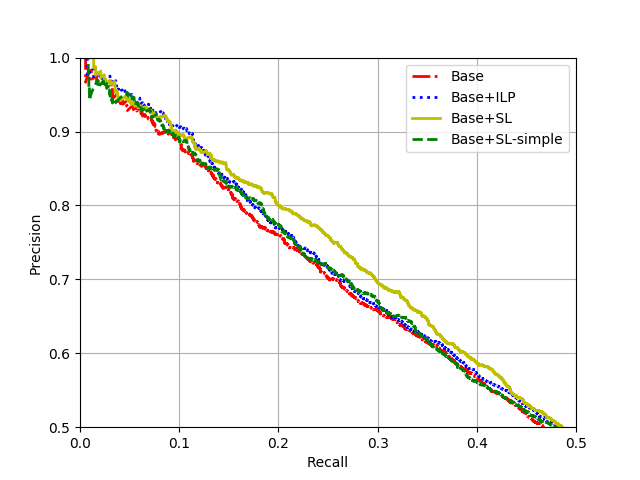
\includegraphics[width=5.5cm]{./result-figure/DBpedia-CNN-result.png}
		%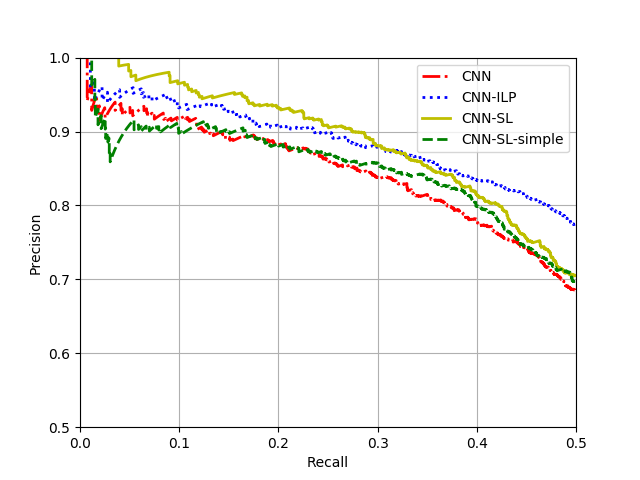
\includegraphics[width=3.5cm]{./result-figure/Chinese-CNN-result.png}
		\caption{Performance on English Dataset}
		\label{fig:dbpedia}
	\end{minipage}
	\begin{minipage}[t]{0.45\textwidth}
		\centering
		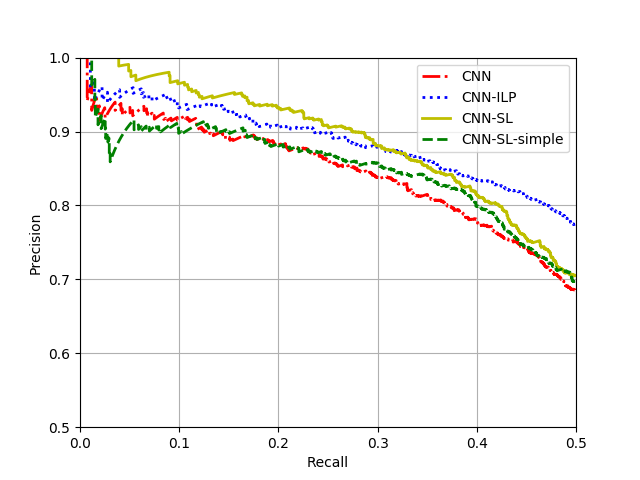
\includegraphics[width=5.5cm]{./result-figure/Chinese-CNN-result.png}
		\caption{Performance on Chinese Dataset}
		\label{fig:chinese}
	\end{minipage}
\end{figure}

\paragraph{Compare with Base Model}
%Compare the semantic loss method and the base model (clear improvement).
As shown in Fig.~\ref{fig:dbpedia} and Fig.~\ref{fig:chinese}, by encouraging the base relation extractor to make predictions that are consistent to our constraints, our \SL method clearly improves the baseline relation extractor in both datasets.
%compared with the baseline, our framework performs consistently better in the DBpedia dataset and Chinese dataset. 
%In order to father demonstrate the semantic loss term helps to encode the constraints into relation extraction model, we count the tuple pairs that violates relation constraints introduced in Sec.~\ref{sec:constraints}, the results is show in Table ~\ref{table:violate-count}.
%IPE:  473.0 WPC:  440.0 CPNI:  273.0 CNN_C:  2123.0 SL_C:  2209.0

%In order to study how our framework improves the performances on the DBpedia dataset and the Chinese dataset, we further dig into the predictions of Base Model and SL Model, we find that our SL model corrects the Base Model's predictions to satisfy the constraints.
Take $<$\emph{Center For Responsible Lending, North Carolina}$>$ and $<$\emph{Meredith College, North Carolina}$>$ as an example.
\base outputs relations \emph{Location} and \emph{CoachedTeam} for these two entity pairs, and our \SL model predicts \emph{Location} and \emph{State} instead.
Note that \emph{Location} requires its object to be a \underline{place}, and \emph{CoachedTeam} expects its object to be a \underline{team}, so there exists a conflict between the two predictions.
\base confuses \emph{CoachedTeam} with \emph{State} since many team names are the same as their state names, and these two relations sometimes share similar expressions in the contexts. 
However, with the help of relation constraints during training, our semantic loss term identifies the conflict and thus encourages the base extractor to focus more on the textual clues that can differentiate these two relations.
% \emph{CoachedTeam}.
%and our SL Model eliminates the conflict through automatically learning constrain knowledge when training. 
%28 8 28 45 

\paragraph{Compare with ILP Method}
%Compare the semantic loss method and ILP.
%NOTE: clw also use cardinality constraints
%We use the same constraints information as the \ILP method of \cite{chen2014encoding}, and Figure ~\ref{fig:dbpedia} and Figure ~\ref{fig:chinese} shows that our SL method delivers superior performance compared to \ILP method in both DBpedia dataset and Chinese dataset.
As shown in Fig.~\ref{fig:dbpedia}, in the English dataset,
\SL gets a comparable performance with \ILP in the high precision region, and performs better than \ILP after 0.15 recall.
We think the performance improvement comes from the fact that \SL functions during training and \ILP only acts as a post-processor.
Therefore, \SL can encourage the base model to find more textual clues when detecting conflicts, while \ILP can only find the most probable relation assignment that satisfies the constraints based on the output scores of the base model, which will possibly drop some high-score predictions and thus still leave the correct relation with a low score.

%For the Chinese dataset, as shown in Fig. ~\ref{fig:chinese}, we can see that \SL performs better in the high precision region.
As for the Chinese dataset, as shown in Fig.~\ref{fig:chinese}, we can see that \SL obtains superior performance in the high precision region, but \ILP performs better in the lower precision region.
%which is also caused by the fact that \ILP tend to leave the predictions corrected by the constraints with low scores.
%However, we find that the constraints in Chinese are more effective than that in the English dataset, which leads to more corrections of the \ILP method.
This is because that the constraints in Chinese are more effective than that in the English dataset, which leads to more corrections of the \ILP method.
Therefore, since \ILP tends to leave the predictions corrected by the constraints with lower scores, a large fraction of the correct predictions gather around the lower score region, which leads to higher precision of the \ILP curve in the high recall region.


%For DBpedia dataset, our method's performance is over \ILP method almost on all precision point. We think this is mainly because \ILP is a post-processing method which choose the most possible prediction that satisfy the constraints from the top three candidate results for every entity pairs, and this would drop some high score predictions, so for the high precision point, our SL method have better performance for both DBpedia dataset and Chinese Dataset. We also find that when recall in (0.3, 0.5), the \ILP is better than our SL method for Chinese Dataset, we think this is because adding constraints for Chinese dataset is much better than DBpedia dataset, the \ILP would drop more high score predictions and the right prediction corrected by \ILP is more likely appear at recall range (0.3, 0.5).


%and Fig.~\ref{fig:chinese}, when using the same constraints and base model, our \SL method is competitive to \ILP, and sometimes even performs better.

In practice, we usually require high-confidence extraction results, the performance of the high-precision region of the PR curve is more important than the low-precision one.
Further, recall that different from \ILP, \SL does not introduce extra cost during prediction.
These experiments indicate that \SL method is more effective than \ILP in practice.
% the performance of high precision in PR curve is more important that the low precision, so totally our SL model gets superior performance than \ILP.
\paragraph{Compare with Simplified Semantic Loss}
%Compare the semantic loss method and the simplified semantic loss.
%Both on PR-curve, and on time.
%To reduce the time cost brought by semantic loss, as described in Sec.~\ref{Sec:simple_SL}, we simplify the calculation of our loss term by only using a subset of relation assignments.
%choosing some constraints from C in ~\ref{seq:semantic_loss} as new $\bm{C'}$, the $ \bm{C'} $ includes one most related constraint with the gold information of tuple pairs and 5 random sampling constraints, then we get the simplified semantic loss $ L^{s}_{simple}(\bm{C'}, \bm{p}) $ as follows:

%\begin{equation}
%\label{seq:semantic_loss_simple}
%L^{s}_{simple}(\bm{C'}, \bm{p}) = -log\sum\limits_{\bm x\models\bm{C'}}\prod\limits_{i:\bm x\models X_i}p_i\prod\limits_{i:\bm x\models \neg X_i}(1-p_i)
%\end{equation}

We also show the performance of our simplified semantic loss in Fig.~\ref{fig:dbpedia} and Fig.~\ref{fig:chinese} (\SLsimple).
We can see that, while inferior to \SL, \SLsimple also improves \base by a clear margin, and it is also comparable to \ILP in the English dataset.
In our experiments, compared to the original \SL method, \SLsimple reduces the extra training time introduced by calculating the semantic loss by 7 times in the English dataset, and 3 times in the Chinese dataset, which has less constraints than those in the English dataset.
%And both in DBpedia dataset and Chinese dataset the simplified semantic loss have improvement over Base Model, especially in DBpedia, it has comparable result with \ILP.
This indicates that \SLsimple acts as a good balance of the trade-off between extraction quality and extra training time.



\section{Conclusion}
%Describe contribution, experimental results (effectiveness of semantic loss method), possibly future work.
In this paper, we introduced a semantic loss for \RE to help resolve the conflicts to type and cardinality constraints among local relation predictions,
which is adapted to most existing relation extractors.
Our method does not bring extra cost during prediction,
and the experiments show that our method consistently improves the performance of the base relation extractor by a clear margin. 
%and we get a clear improvements compared with the base model. 
%into the relation extractors through the semantic loss framework to help resolve the disagreements among local relation predictions, and we get a clear improvements compared with the base model. 
%Our method automatically learns the constraints during training, and does not incurs extra costs in testing. 
%Further, our method prefers to get high-confidence extraction results comparing with \ILP, this is crucial in practice.
%And our method could generally incorporate with most relation extractor models and help them to resolve the disagreements among local relation predictions.

\bibliography{emnlp2018}
\bibliographystyle{acl_natbib_nourl}


\end{document}
